%%%%%%%%%%%%%%%%%%%%%%%%%%%%%%%%%%%%%%%%%%%%%%%%%%%%%%%%%%%%%%%%%%%%%%%%%%%%%%%%
%2345678901234567890123456789012345678901234567890123456789012345678901234567890
%        1         2         3         4         5         6         7         8

%\documentclass[letterpaper, 10 pt, conference]{ieeeconf}  % Comment this line out
                                                          % if you need a4paper
\documentclass[a4paper, 10pt, conference]{ieeeconf}      % Use this line for a4
                                                          % paper

\IEEEoverridecommandlockouts                              % This command is only
                                                          % needed if you want to
                                                          % use the \thanks command
\overrideIEEEmargins
% See the \addtolength command later in the file to balance the column lengths
% on the last page of the document
% packages
% The following packages can be found on http:\\www.ctan.org
\usepackage{graphicx} % for pdf, bitmapped graphics files
\usepackage{epsfig} % for postscript graphics files
\usepackage{mathptmx} % assumes new font selection scheme installed
\usepackage{times} % assumes new font selection scheme installed
\usepackage{amsmath} % assumes amsmath package installed
\usepackage{amssymb}  % assumes amsmath package installed
\usepackage{hyperref}
\usepackage{listings}

\graphicspath{ {files/} }

\title{\LARGE \bf Using GEM5 for Architecture Exploration in Multi-Core Processors}

\author{Christopher Ohara (1322884) \\
Erik Wouters (1325892)
}

\begin{document}

\maketitle
\thispagestyle{empty}
\pagestyle{empty}

%%%%%%%%%%%%%%%%%%%%%%%%%%%%%%%%%%%%%%%%%%%%%%%%%%%%%%%%%%%%%%%%%%%%%%%%%%%%%%%%
\begin{abstract}
In this report the multi-core optimization of an EEG application written in C is explored using simulated ARM A9 and A15 cores on the GEM5 platform. The impact of different design parameters such which cores to use and the L1 and L2 cache sizes. The optimization requirement is to minimize execution time while taking the consequences with respect to chip area and energy consumption into consideration by comparing the Energy Delay Area Product (EDAP).

\end{abstract}

%%%%%%%%%%%%%%%%%%%%%%%%%%%%%%%%%%%%%%%%%%%%%%%%%%%%%%%%%%%%%%%%%%%%%%%%%%%%%%%%
\section{Introduction}
Using GEM5\cite{gem5}, multi-core processors can be emulated allowing analysis and comparison by adjusting different parameters and factors. This project is primarily designed to enable users to create optimized ARM processors using a simulator. A broad range of algorithms can be utilized or created. The implementation also consists of using OpenMP\cite{openmp}, an API for shared-memory parallel programming.

Throughout the report there are shown tables and
graphs of which the data for them is sourced from a
stats.txt file that GEM5 is outputting. In such a file,
the following keys were searched in order to study performance:


Throughout this report there are tables and figures which have been created using the \texttt{stats.txt} output of the GEM5 simulator. The following keys from the file are the most notable:
\begin{itemize}
    \item sim\_seconds: Number of seconds simulated
    \item system.cpu.icache.overall\_mshr\_miss\_rate::total
    \item system.cpu.dcache.overall\_mshr\_miss\_rate::total
    \item system.l2.overall\_miss\_rate::total
    \item system.cpu.icache.overall\_avg\_mshr\_miss\_latency::total
    \item system.cpu.dcache.overall\_avg\_mshr\_miss\_latency::total
    \item system.l2.overall\_avg\_miss\_latency::total
\end{itemize}

The miss rates and miss latencies are determined from the Miss Status Handling Registers (MSHR). These latencies and miss rates provide insight in how long the processor has to stall when there is a cache miss.

%These keys can be used to compute the Average memory access time (AMAT) using the formula
%
%\[
%    AMAT_{L1} = Hit Time_{L1} + Miss Rate_{L1} \dot \]\[
%    (Hit Time_{L2} + Miss Rate_{L2} + Miss Penalty_{L2})
%\]

\section{ARM A9}

\subsection{L1 Cache Size}

To measure the impact of the L1 cache size on the execution time of the EEG application the L2 cache has been disabled and the L1 instruction and data cache size was varied between $64B$ and $64kB$ in steps of powers of two. This allows for performance analysis with respect to adjustments in cache sizes. Table \ref{tab:A9_L1} and \ref{fig:ex1_1} show the performance of the EEG application. It can be observed that a bigger cache size results in a smaller run-time. This is to be expected because with a bigger cache there will be fewer compulsory cache misses. The steepest point of the graph is found at around $512B$. The improvement slows down above $2kB$, so for this application having a L1 cache size of about $1kB$ to $2kB$ would give good results. If the cache size would be bigger the speedup would be cancelled out by the increase in area and energy, so the EDAP would not increase.

\begin{table}[h]
\caption{ARM A9 - L1 Cache Size vs. Total Ticks}
\label{tab:A9_L1}
\begin{center}
\begin{tabular}{|c||c|}
\hline
Cache Size & Total Ticks\\
\hline
64B & 4.2896E+12\\
\hline
128B & 4.19046E+12\\
\hline
256B & 3.66132E+12\\
\hline
512B & 2.71066E+12\\
\hline
1kB & 1.46311E+12\\
\hline
2kB & 1.00441E+12\\
\hline
4kB & 6.85485E+11\\
\hline
8kB & 6.36708E+11\\
\hline
16kB & 5.92753E+11\\
\hline
32kB & 5.48413E+11\\
\hline
64kB & 5.43378E+11\\
\hline

\end{tabular}
\end{center}
\end{table}

\begin{figure}[thpb]
\centering
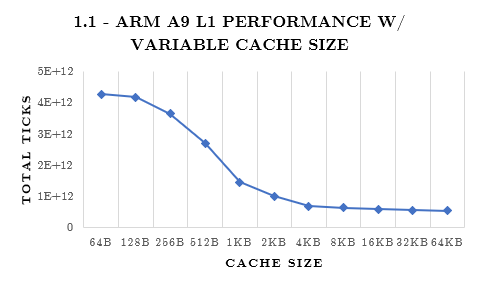
\includegraphics[scale=.5]{ex1_1.png}
\caption{Impact on number of ticks by varying the L1 cache size}
\label{fig:ex1_1}
\end{figure}

\subsection{Associativity Level}

To determine the impact of the associativity the L1 instruction and data cache size is set to a constant $2kB$, while still keeping the L2 cache disabled (to restrict the number of free variables). Then the associativity is varied between $1$ and $8$ in steps of powers of two because if non-powers of two are used the tag sizes will not line up nicely. Table \ref{tab:ticks_assoc} and \ref{fig:ticks_assoc} show that increasing the associativity from one to two gives the best relative speedup, while increasing it further provides a more marginal speedup.

\begin{table}[h]
\caption{ARM A9 - L1 Associativity vs. Total Ticks}
\label{tab:ticks_assoc}
\begin{center}
\begin{tabular}{|c||c|}
\hline
Associativity & Total Ticks\\
\hline
1 & 1.00454E+12\\
\hline
2 & 7.27428E+11\\
\hline
4 & 6.87746E+11\\
\hline
8 & 6.83377E+11
\\
\hline
\end{tabular}
\end{center}
\end{table}


\begin{figure}[thpb]
\centering
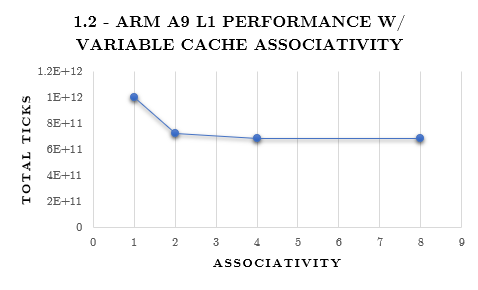
\includegraphics[scale=.5]{ex1_2.png}
\caption{Impact on number of ticks by varying the associativity level}
\label{fig:ticks_assoc}
\end{figure}

\subsection{L2 Cache Size}

To explore the differences between varying the L1 and L2 cache sizes, a direct mapped L2 cache size is varied while the L1 cache sizes are now held constant. Table \ref{tab:A9_size} and Figure \ref{fig:A9_size} show a very linear decrease in the execution time when the L2 cache size is increased logarithmically. This implies that the more L2 cache is added, the lower the execution time. This relation will come to a halt when the cache size approaches the size of the input data however.

\begin{table}[h]
\caption{ARM A9 - L1 Cache Size vs. Total Ticks}
\label{tab:A9_size}
\begin{center}
\begin{tabular}{|c||c|}
\hline
Cache Size & Total Ticks\\
\hline
2kB & 1.03179E+12 \\ \hline
4kB & 9.60558E+11 \\ \hline
8kB & 9.08990E+11 \\ \hline
16kB & 8.55049E+11 \\ \hline
\end{tabular}
\end{center}
\end{table}

\begin{figure}[htb]
\centering
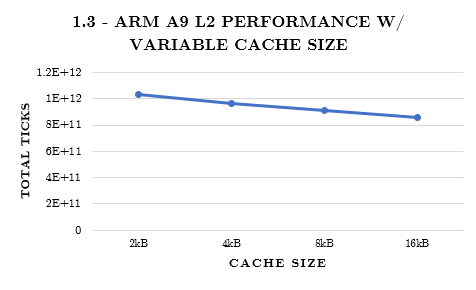
\includegraphics[scale=.5]{ex1_3.png}
\caption{Impact on number of ticks by varying the L2 cache size}
\label{fig:A9_size}
\end{figure}

%\pagebreak

\section{ARM A15}

GEM5 can simulate very detailed models of processors. So far a model close to the ARM A9 core has been simulated. In the next simulation a model close to the ARM A15 core has been used.

The ARM A15 is simulated by using an out-of-order CPU that utilizes decoding, issuing, fetching and dispatching 3 instructions per cycle. It also incorporates two integer ALUs, one integer divider, one integer multiplier and a read/write port.

\begin{table}[h]
\caption{ARM A15 - L1 Cache Size and Total Ticks}
\label{tab:A15}
\begin{center}
\begin{tabular}{|c||c|}
\hline
Cache Size & Total Ticks\\
\hline
64B & 4.18925E+12
\\
\hline
128B & 4.13002E+12
\\
\hline
256B & 3.59686E+12
\\
\hline
512B & 2.62578E+12
\\
\hline
1kB & 1.36592E+12
\\
\hline
2kB & 8.97505E+11
\\
\hline
4kB & 5.56189E+11
\\
\hline
8kB & 4.9869E+11
\\
\hline
16kB & 4.49761E+11
\\
\hline
32kB & 3.95024E+11
\\
\hline
64kB & 3.87966E+11
\\
\hline

\end{tabular}
\end{center}
\end{table}

\begin{figure}[thpb]
\centering
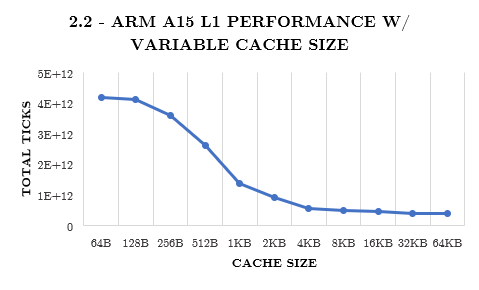
\includegraphics[scale=.5]{ex2_2.png}
\caption{Impact on number of ticks by varying the cache size}
\label{figure2_2}
\end{figure}

\section{Experimenting with OpenMP, multithreading and multi-core architectures}

The test code for the EEG application has been modified to run on a multi-core platform using the OpenMP API. For-loops that have no dependencies between iterations have been preceded by a statement to run the iterations in parallel. This has been done for every for-loop in the application and the validity of the multi-core program has been tested by compiling it natively and by running a simulation on the heterogeneous platform.

An example of a modification is shown in the snippet below:

\begin{lstlisting}
#pragma omp parallel for
for (i = 0; i < CHANNELS; i++) {
printf("Running channel %d...\n", i);
run_channel(DATAPOINTS, x[i], features[i]);
}
\end{lstlisting}

\section{Heterogeneous Platform A15-A15-A9-A9}
As a final experiment a heterogeneous multi-core platform consisting of two A15 cores and two A9 cores has been simulated. Each of the cores has a private L1 cache and the four cores use a shared L2 cache.

The optimized values for the L1 cache have been chosen by finding the inflection point of the graphs in Figures \ref{fig:ex1_1} and \ref{fig:ticks_assoc}. For both the A15 and the A9 cores the optimal size of the cache is $1kB$. At the infliction point the trade-off between cost for larger cache and speed-up in number of cycles is optimal. The associativity is chosen as 2-way, because we see a large performance increase when the associativity is increased from 1 to 2, but the graph of Figure \ref{fig:ticks_assoc} becomes very flat after that point.

For the L2 cache we can see in Figure \ref{fig:A9_size} that the larger this cache is, the faster the EEG application will run. $16kB$ is a feasible size for the L2 cache of the heterogeneous platform.

This platform performed 5.81 times faster on the EEG application than the single A9 core version and 1.27 times faster than the 3-core homogeneous A9 platform with comparable cache sizes.

%%%%%%%%%%%%%%%%%%%%%%%%%%%%%%%%%%%%%%%%%%%%%%%%%%%%%%%%%%%%%%%%%%%%%%%%%%%%%%%%


\begin{thebibliography}{99}

\bibitem{gem5} Nathan Binkert, Bradford Beckmann, Gabriel Black, Steven K. Reinhardt, Ali Saidi, Arkaprava Basu, Joel Hestness, Derek R. Hower, Tushar Krishna, Somayeh Sardashti, Rathijit Sen, Korey Sewell, Muhammad Shoaib, Nilay Vaish, Mark D. Hill, and David A. Wood. 2011. The gem5 simulator. SIGARCH Comput. Archit. News 39, 2 (August 2011), 1-7. DOI=\url{http://dx.doi.org/10.1145/2024716.2024718}

\bibitem{openmp} Dagum, Leonardo, and Ramesh Menon. "OpenMP: an industry standard API for shared-memory programming." Computational Science \& Engineering, IEEE 5.1 (1998): 46-55.



\end{thebibliography}






%\newpage
\onecolumn
\section*{APPENDIX}

\begin{figure}[thpb]
\centering
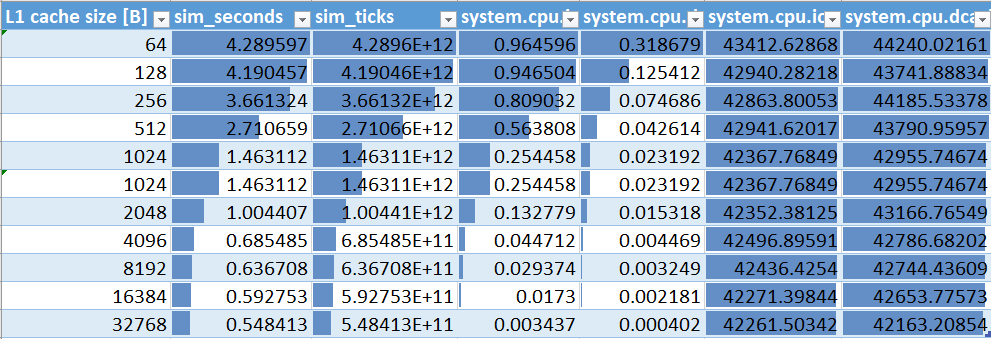
\includegraphics[scale=0.7]{Figures/assignment1_1_table.png}
\caption{A9: L1 cache size in bytes vs. sim\_seconds, sim\_ticks, L1 instruction cache miss rate, L1 data cache miss rate, L1 instruction cache average miss latency and L1 data cache average miss latency}
\label{Afigure1_1}
\end{figure}

\begin{figure}[thpb]
\centering
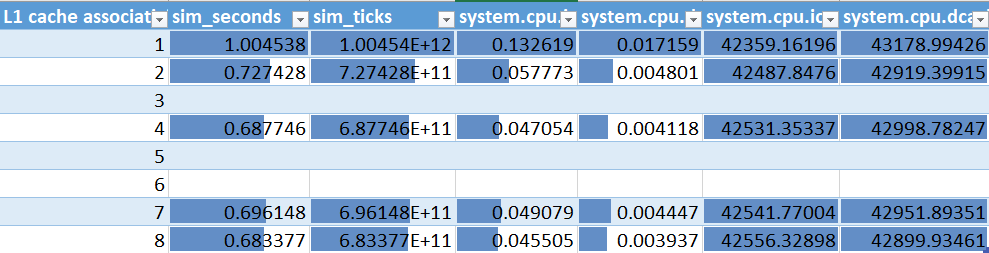
\includegraphics[scale=0.7]{Figures/assignment1_2_table.png}
\caption{A9: L1 cache associativity vs. sim\_seconds, sim\_ticks, L1 instruction cache miss rate, L1 data cache miss rate, L1 instruction cache average miss latency and L1 data cache average miss latency}
\label{Afigure1_2}
\end{figure}

\begin{figure}[thpb]
\centering
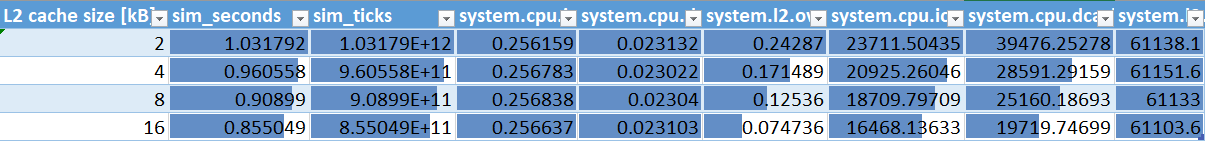
\includegraphics[scale=0.572]{Figures/assignment1_3_table.png}
\caption{A9: L2 cache size vs. sim\_seconds, sim\_ticks, L1 instruction cache miss rate, L1 data cache miss rate, L2 cache miss rate, L1 instruction cache overall average miss latency, L1 data cache overall average miss latency and L2 cache average miss latency}
\label{Afigure1_3}
\end{figure}

\begin{figure}[thpb]
\centering
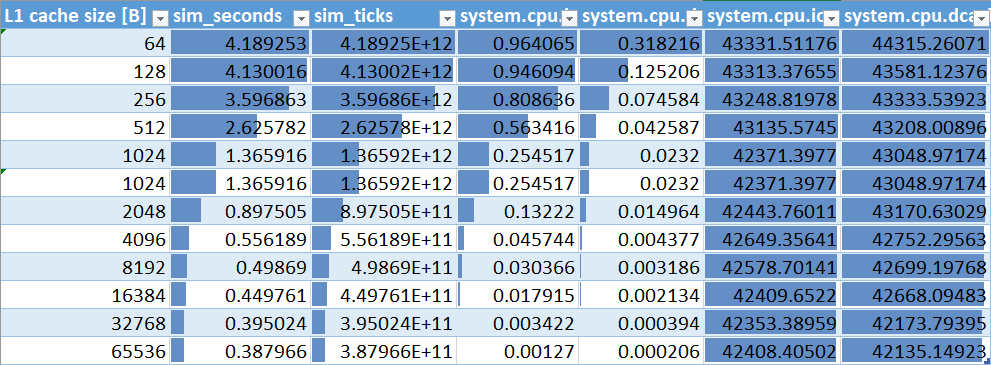
\includegraphics[scale=0.7]{Figures/assignment2_2_table.png}
\caption{A15: L1 cache size in bytes vs. sim\_seconds, sim\_ticks, L1 instruction cache miss rate, L1 data cache miss rate, L1 instruction cache average miss latency and L1 data cache average miss latency}
\label{Afigure2_2}
\end{figure}

\end{document}
